\section{Objectives and specification mapping}
Lab 4 (PDF pages 17--20) compares diffusion geometry, junction capacitance and a constant-capacitance approximation for a three-input NAND. Step 1 requests ACM=2/3 comparison, Step 2 asks for node-capacitance calculations, and Step 3 replaces the junction contribution by $(C_{\max}+C_{\min})/2$.

This implementation completes explicit AD/AS/PD/PS sensitivity tests, numerical junction-capacitance extraction, node-capacitance sums and fixed-C simulation. The supplied model is encrypted and its process design rules are unavailable, so direct modification of its ACM setting and foundry-qualified HDIF are not claimed. This is a circuit-simulation adaptation with stated limits; no layout, DRC, LVS or extracted-layout verification is performed.

\section{Circuit and geometry derivation}
Three PMOS devices form the parallel pull-up and three NMOS devices form the series pull-down. Every device has $W=1.8\,\mu$m and $L=0.25\,\mu$m. Input A switches while B=C=1, with a 10 fF external load. A W/L-only model-default branch provides an additional reference.

The teaching geometry uses $H=0.27\,\mu$m as an explicit sensitivity-test assumption, not as this model's minimum design rule. The handout ACM=2 equations give $A=2HW=0.972\,\mu$m$^2$ and $P=2(2H+W)=4.68\,\mu$m. For the ACM=3 geometry, an unshared terminal has $A=2HW$ and $P=4H+W=2.88\,\mu$m; a shared terminal has $A=HW=0.486\,\mu$m$^2$ and $P=2H=0.54\,\mu$m. Devices A/B/C use the sharing patterns associated with GEO=2/3/1. These areas and perimeters are explicit instance values, rather than an assumed change to hidden model options. NRD=NRS=H/W=0.15.

A generic junction equation is
\[ C_j(V)=\frac{A C_{j0}}{(1+V/\Phi)^m}+\frac{P C_{jsw0}}{(1+V/\Phi_{sw})^{m_{sw}}}. \]
The encrypted model does not expose a verified coefficient set, so no foundry-coefficient hand calculation is invented. Instead, off-channel NMOS/PMOS drain and source tests apply a 1 V small-signal excitation at 1 MHz. A zero-area, zero-perimeter reference at the same bias removes the background contribution: $C_j=-\Delta\operatorname{Im}(I)/(2\pi f)$. Reverse-bias samples are 0, 0.25, 0.5, 0.75 and 1 V.

\section{Simulation setup and measurement definitions}
The separately supplied MOS model is evaluated at 1.0 V and $27\,^{\circ}$C, retaining the handout topology and the comparison conditions below. One volt is a simulation setting, not a device rating established by available model documentation. Numerical results from the handout's older processes are not acceptance targets for this model.

HSPICE S-2021.09 runs with RUNLVL=6. Tables use actual native measurements and figures use actual printed numerical traces. Every variant resets all swept parameters and temperature, avoiding inherited settings from an earlier variant. Completed solutions and measurements do not establish process reliability. Internal warnings in encrypted model blocks remain incompletely visible.
The input swings 0--1 V with 100 ps PULSE rise/fall parameters and a 20 ns period. Transient duration is 40 ns, printed every 2 ps. Propagation delays use 50\% input/output crossings; output transitions use 10--90\% crossings.

\section{Measured results}
Three netlists and seven cases completed with no errors or failed measurements. Geometry-comparison timing values below are in ps.

\begin{center}\small
\begin{tabular}{lllll}
\toprule
Geometry & $t_{pHL}$ & $t_{pLH}$ & $t_r$ & $t_f$ \\
\midrule
Model default & 70.30 & 127.58 & 165.68 & 92.29 \\
Unshared & 84.81 & 160.89 & 230.57 & 123.18 \\
Shared & 75.74 & 138.84 & 186.59 & 101.34 \\
\bottomrule
\end{tabular}
\end{center}
\begin{figure}[htbp]
\centering
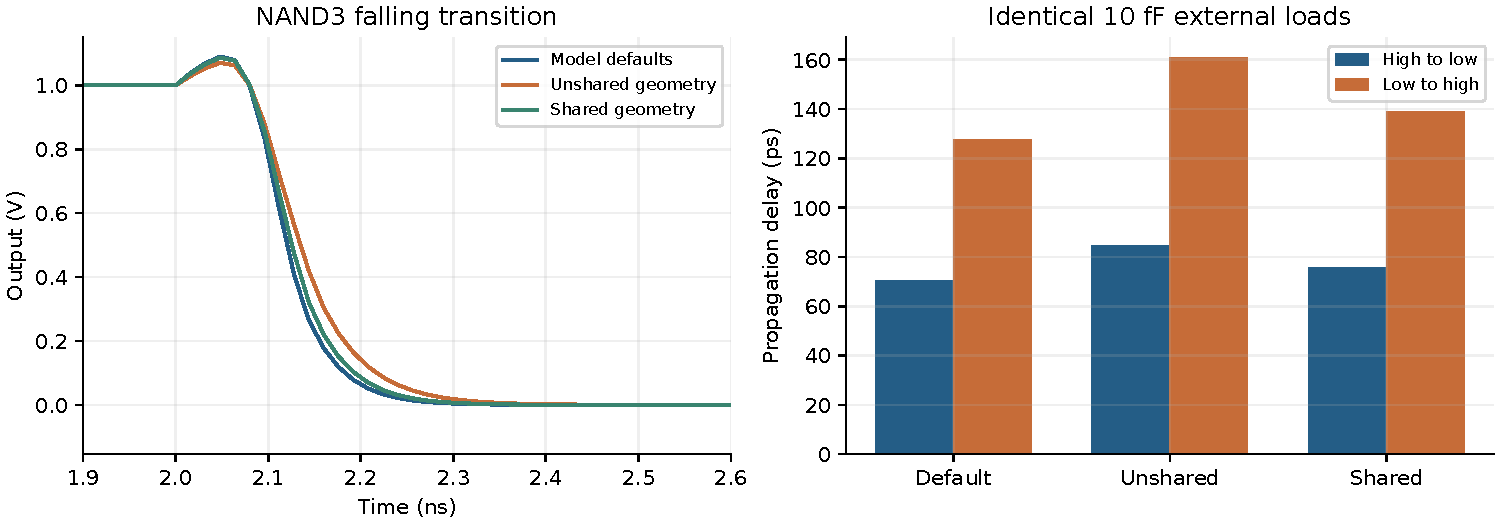
\includegraphics[width=\linewidth]{figures/diffusion_geometry.pdf}
\caption{Measured NAND delay and falling waveforms for explicit geometries.}
\end{figure}
\section{Node capacitance and fixed-C approximation}
For the unshared geometry the output junction contribution is $3C_{p,d}+C_{n,d}$; n1 and n2 sum the adjacent NMOS source and drain contributions. Shared geometry sums the appropriate terminal types. Each terminal first takes $(C_{\max}+C_{\min})/2$ over the bias sweep; node sums are listed in fF. Fixed-C branches set AD/AS/PD/PS to zero before adding these capacitors, avoiding double counting. Intrinsic channel capacitances, other model behavior and the external 10 fF load remain.

\begin{center}\small
\begin{tabular}{lll}
\toprule
Geometry mode & Node & C (fF) \\
\midrule
2 & y & 8.6305 \\
2 & n1 & 4.1352 \\
2 & n2 & 4.1352 \\
3 & y & 3.3841 \\
3 & n1 & 0.5276 \\
3 & n2 & 0.5276 \\
\bottomrule
\end{tabular}
\end{center}
\begin{center}\small
\begin{tabular}{lll}
\toprule
Mode & $t_{pHL}$ dependent/fixed (ps) & $t_{pLH}$ dependent/fixed (ps) \\
\midrule
2 & 84.85 / 88.32 & 161.01 / 171.80 \\
3 & 75.75 / 78.30 & 139.00 / 145.06 \\
\bottomrule
\end{tabular}
\end{center}
\begin{figure}[htbp]
\centering
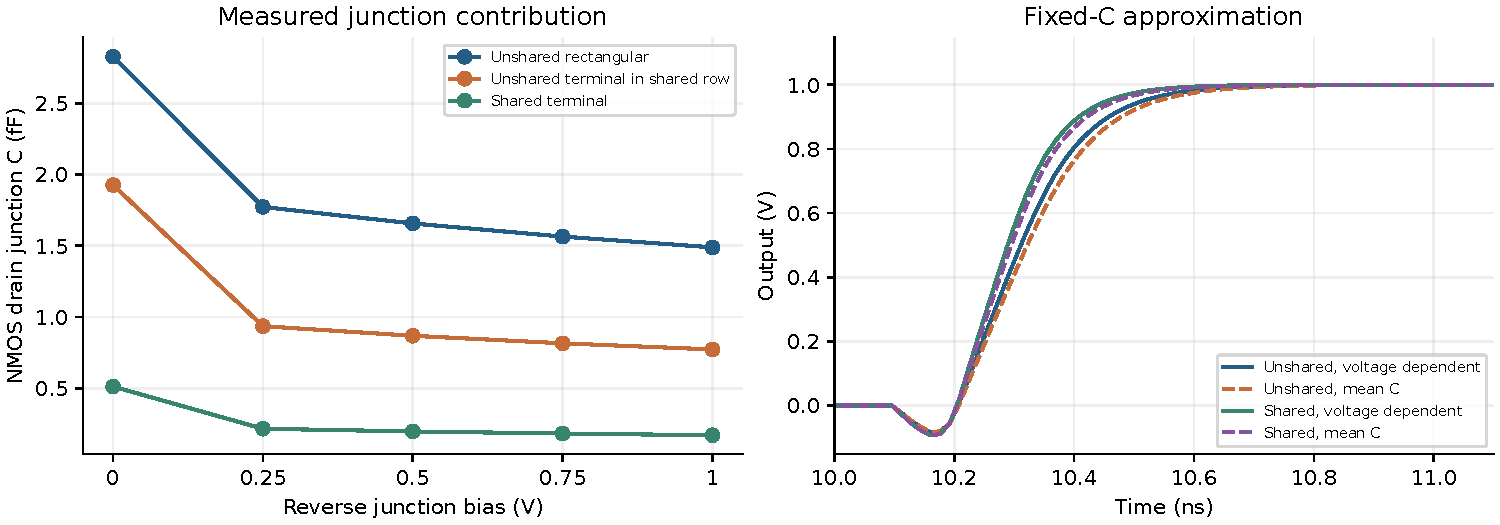
\includegraphics[width=\linewidth]{figures/junction_capacitance.pdf}
\caption{Bias-dependent junction contribution and the fixed-mean-C rising waveform comparison.}
\end{figure}
\section{Discussion and limitations}
Shared diffusion reduces area and perimeter and therefore lowers added junction loading and delay in this experiment. A constant average capacitance cannot track the changing junction bias throughout a transition. Falling/rising delay errors are 4.09\%/6.70\% for unshared geometry and 3.36\%/4.36\% for shared geometry. All fixed-C delays are slightly larger; the mean-C model is not pointwise equivalent.

These results validate the circuit consequences of the handout geometry equations and a measured mean-C approximation. Literal ACM=2/3 model-option selection, foundry HDIF and a full coefficient-based hand calculation remain unverified. The model-default branch must not be described as a known ACM=2 configuration.

\section{Reproducibility files}
Netlists: \texttt{01\_geometry.sp}, \texttt{02\_junction\_capacitance.sp}, \texttt{03\_constant\_capacitance.sp}. Add the local model configuration at the marked comment before execution; model files and paths are omitted from the public files.

The results directory contains all case measurements, derived metrics, the specification manifest and representative waveform CSVs. Waveforms retain at most 2501 uniformly selected samples; measurements are not downsampled. Full listings remain local.
